\textbf{Problem 2.  Iterative Methods: Jacobi, G-S, Multigrid}

We wish to solve the Poisson equation:
\begin{align}
    -\nabla^2\phi(x,y) = f
\end{align}

\begin{enumerate}[label=(\roman*),leftmargin=*,itemsep=0mm]
    
    \item The matrix forms of the Jacobi and Gauss-Siedel iterations are, respectively:
    \begin{align}
        \mathbf{u}^{r+1} &= (I-D^{-1}A)\mathbf{u}^r + D^{-1}f \\
        \mathbf{u}^{r+1} &= (D-L)^{-1}U\mathbf{u}^r + (D-L)^{-1}f
    \end{align}
    
    Discretization of the Poisson equation gives us:
    \begin{align}
        \nabla^2\phi(x,y) &= \frac{\partial^2\phi}{\partial{x^2}} + \frac{\partial^2\phi}{\partial{y^2}} \nonumber \\
        &= \frac{\phi_{i+1,j}+\phi_{i-1,j}-2\phi_{i,j}}{\Delta x^2}
        + \frac{\phi_{i,j+1}+\phi_{i,j-1}-2\phi_{i,j}}{\Delta y^2}
    \end{align}
    
    Given that we have $N^2$ nodes on the computational grid, where $N = 6n + 1 \> \forall \> n\in \mathbb{N}$.  Therefore, representing the nodes of the computational grid by $(i,j)$, we have that the for a given $(i,j)$ computational node, where $2 \leq i,j \leq N-1$, the elements of $A$ are, where $k = i + (j-1)N$
    \begin{itemize}[noitemsep,nolistsep]
        \item $a_{k,k} = 4$
        \item $a_{k,k-1} = a_{k,k+1} = a_{k,k-N} = a_{k,k+N} = -1$
    \end{itemize}
    
    When $i=1$ or $i = N$ or $j = 1$ or $j = N$, the elements of $A$ are, where $k = i + (j-1)N$
    \begin{itemize}[noitemsep,nolistsep]
        \item $a_{k,k} = 1$
    \end{itemize}
    
    The elements of $D$ are
    \begin{itemize}[noitemsep,nolistsep]
        \item $d_{k,k} = \dfrac{2}{(\Delta x)^2} + \dfrac{2}{(\Delta y)^2}$
    \end{itemize}
    
    The elements of $L$ are
    \begin{itemize}[noitemsep,nolistsep]
        \item $l_{k,k-1} = l_{k,k-N} = \dfrac{1}{(\Delta x)^2}$
    \end{itemize}
    
    The elements of $U$ are
    \begin{itemize}[noitemsep,nolistsep]
        \item $u_{k,k+1} = u_{k,k+N} = \dfrac{1}{(\Delta x)^2}$
    \end{itemize}
    
    The elements of $f$ are determined by the location of the source blocks (which have 16 possible positions).  Given a source block at position $s = s_1 + 4(s_2-1) \>\forall\> 1 \leq s_1,s_2 \leq 4$ out 16, the following points $f_{i+(j-1)N}$ are set to 1, where $i,j$ are given by
    \begin{itemize}
        \item $ns_1 + 1 \leq j \leq n(s_1+1) + 1$
        \item $ns_2 + 1 \leq i \leq n(s_2+1) + 1$
    \end{itemize}
    
    where $n$, as given above, is defined by $N = 6n + 1 \> \forall \> n\in \mathbb{N}$ given that the computational grid is for $N^2$ nodes.

    \begin{figure*}[h!]
    \centering
    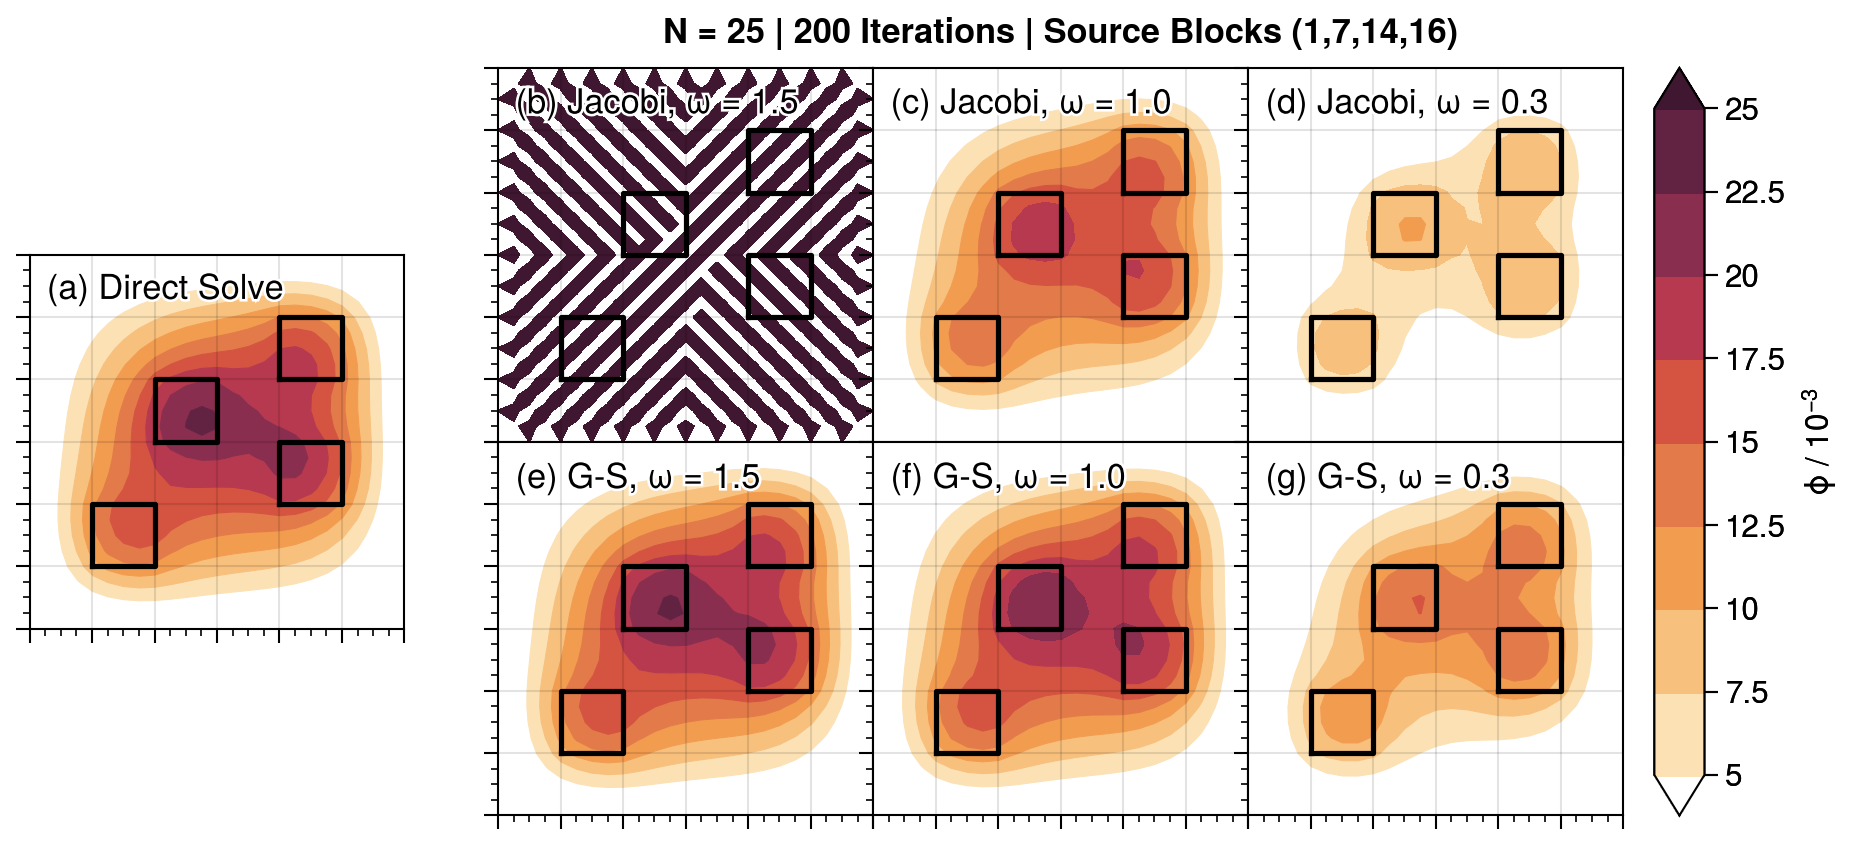
\includegraphics[width=\textwidth]{figures/prj1_qn2_solutions.png}\\
    \caption{We plot here the spatial distribution for $\phi$ derived from (a) the reference solution generated from directly solving the equation $A\mathbf{u} = f$; (b-d) using the Jacobi-iterative solver; (e-g) using the Gauss-Seidel iterative solver, for different relaxation factors (b,e) $\omega=1.5$, (c,f) $\omega=1.0$ and (d,g) $\omega=0.3$.  We see that as $\omega$ increases, the speed at which the solutions converge increase.  However, as can be seen in (b) an over-relaxation of the Jacobi iterative method causes a failure of convergence and the solution blows up.}
    \label{prj1_qn2_sol}
    \end{figure*}
    
    \item We first implement the relaxation scheme using the variable $\omega$.  For the Jacobi, this means transforming Eq. (30) to:
    \begin{align}
        \mathbf{u}^{r+1} &= \omega((I-D^{-1}A)\mathbf{u}^r + D^{-1}f) + (1-\omega) \mathbf{u}^r
    \end{align}
    
    And for the Gauss-Seidel, this means transforming Eq. (31) to
    \begin{align}
        \mathbf{u}^{r+1} &= \omega((D-L)^{-1}U\mathbf{u}^r + (D-L)^{-1}f) + (1-\omega)\mathbf{u}^r
    \end{align}
    
    We then plot, for different values of relaxation factor $\omega$, the spatial distribution of $\phi$ at iteration 200 (Fig. \ref{prj1_qn2_sol}) and the convergence of the Jacobi and G-S solvers (Fig. \ref{prj1_qn2b_converge}).  Our initial condition is to set $\phi=0$ throughout the domain, which is $(x,y) \in [0,1]$.

    \begin{figure*}[h!]
    \centering
    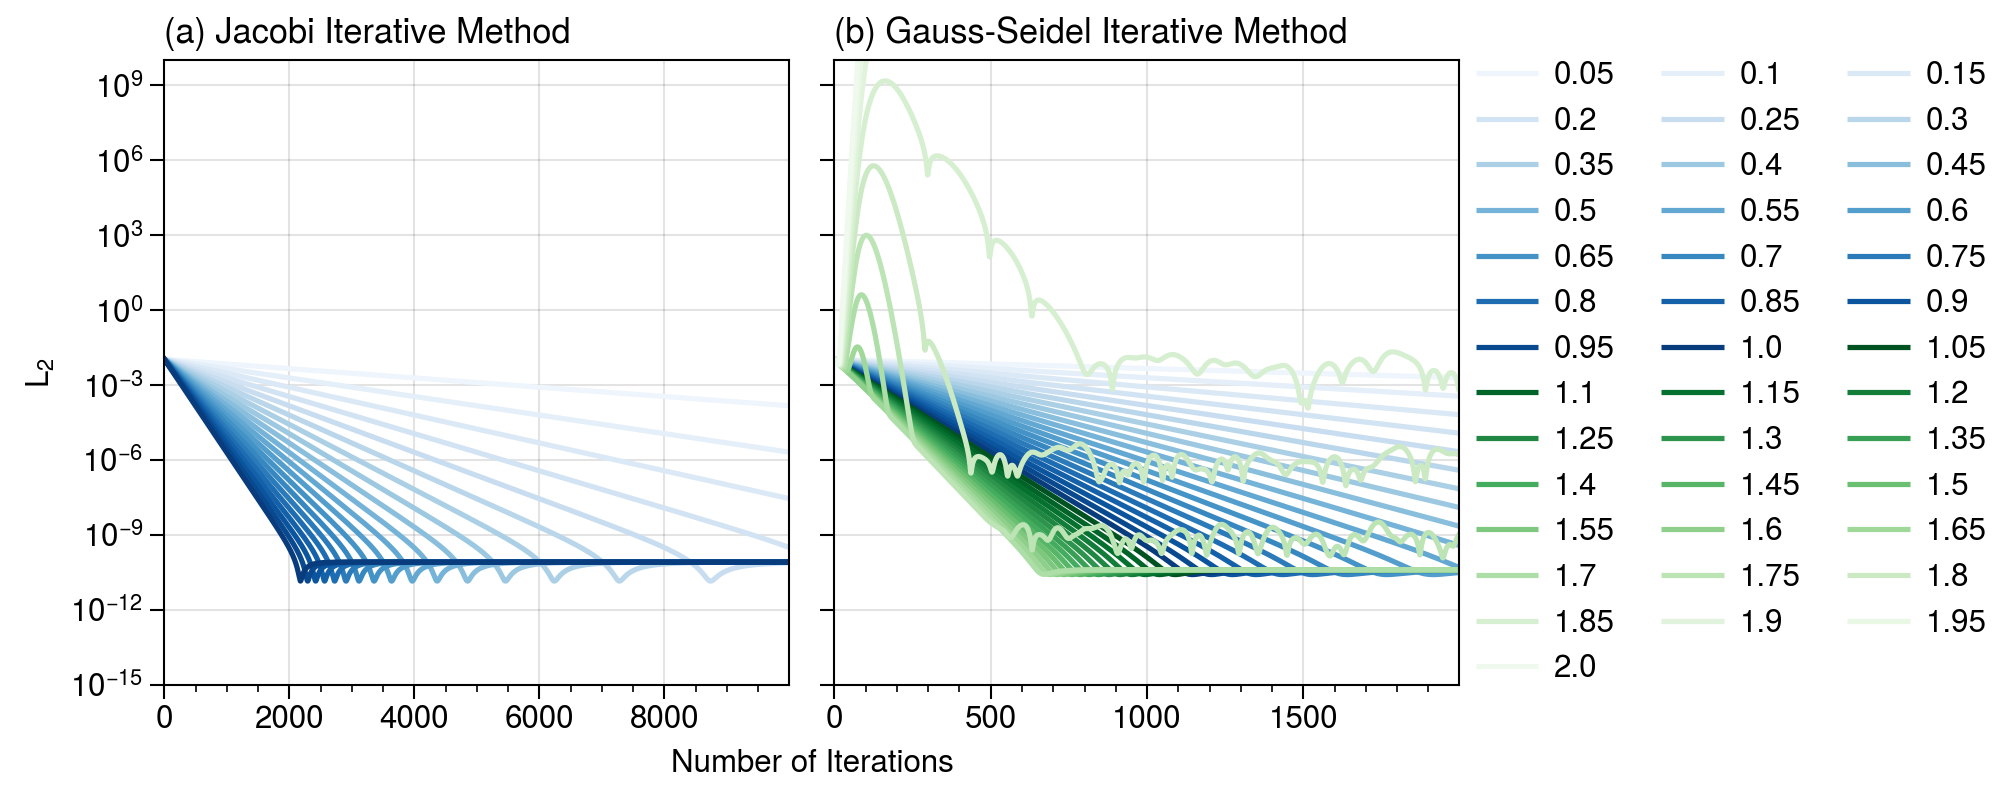
\includegraphics[width=\textwidth]{figures/prj1_qn2b_converge.png}\\
    \caption{The $L_2$ norm of $\phi$ for the (a) Jacobi and (b) Gauss-Seidel iteration as a function of the number of iterations for different relaxation factors $\omega$, where $\omega \in (0,1]$ for the Jacobi and $\omega\in(0,2]$ for the Gauss-Seidel methods.}
    \label{prj1_qn2b_converge}
    \end{figure*}
    
    For the Jacobi iterative method, we see that $\omega = 1$ is the most optimal method for convergence.  However, for the Gauss-Seidel method, things become a bit more complicated.  Although theoretically $\omega$ can go to 2 for the Gauss-Seidel iterative method, we see that this is practically not the case most of the time.  Here, we see that for $\omega \gtrapprox 1.7$, $L_2$ begins to show instability as it converges, with $L_2$ blowing up as $\omega \rightarrow 2$.
    
    We see therefore that the optimal relaxation factor is $\omega \approx 1.7 \pm 0.1$.  Next, we output the gradient at iteration 750 of $N=25$ for $\omega=1.7$.
    
    \begin{lstlisting}
 ------ ------------ ------------ ------------ ------------
  Node      Left        Right        Bottom        Top     
 ------ ------------ ------------ ------------ ------------
  1.0       0.0          0.0          0.0          0.0
  2.0    0.0122496    0.00715823    0.01224     0.00543106
  3.0    0.0243891    0.0144921    0.0243505    0.0108636
  4.0    0.0360682    0.0221708    0.0359625     0.016292
  5.0    0.0465743    0.0303384    0.0463457    0.0216962
  6.0    0.0551794    0.0390685    0.0547578    0.0270368
  7.0    0.0611753    0.0482715    0.0604839    0.0322526
  8.0    0.0643138    0.0575573    0.0632823    0.0372662
  9.0    0.0648678    0.0661676    0.0634521    0.0419991
  10.0   0.0635626    0.0733503    0.0617709    0.0463955
  11.0   0.0611295    0.0784066    0.0590498    0.0504469
  12.0   0.0582652    0.0811326    0.0560855     0.054205
  13.0   0.0552769    0.0818649     0.053285    0.0577673
  14.0   0.0521775    0.0813697    0.0507309    0.0612186
  15.0   0.0488556    0.0803017    0.0483185    0.0645118
  16.0   0.0451946    0.0790181    0.0458536    0.0673012
  17.0   0.0411317    0.0771352    0.0431148    0.0688502
  18.0   0.0366709    0.0739684    0.0398962    0.0683913
  19.0   0.0318686    0.0687154    0.0360414    0.0651714
  20.0   0.0268081    0.0609928    0.0314677    0.0589027
  21.0   0.0215738    0.0509451    0.0261747    0.0498331
  22.0   0.0162358    0.0391958    0.0202373    0.0386868
  23.0   0.0108432    0.0264069    0.0137856    0.0262219
  24.0   0.00542594   0.0132393    0.00698161    0.013193
  25.0      0.0          0.0          0.0          0.0
 ------ ------------ ------------ ------------ ------------
\end{lstlisting}
    
    Which is what was given, except to even higher significant figures.
    
    \item We first test our restriction and prolongation matrices to determine if they are correct (Fig. \ref{prj1_qn2c_testrestrictprolong}).

    \begin{figure*}[h!]
    \centering
    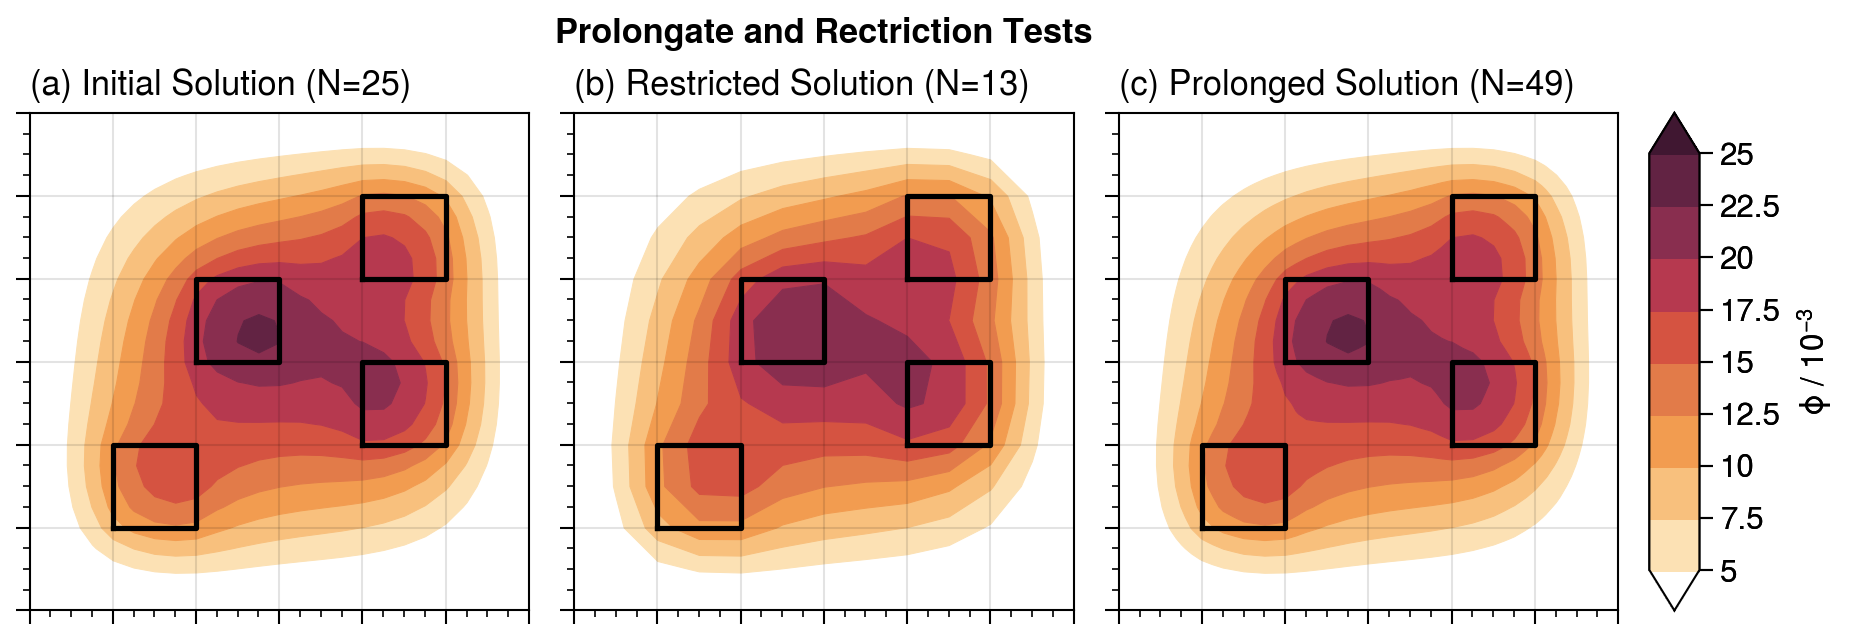
\includegraphics[width=\textwidth]{figures/prj1_qn2c_testrestrictprolong.png}\\
    \caption{We test the relaxation and prolongation matrices we constructed by plotting (a) the initial solution, and the (b) restricted and (c) prolongated solutions found by multiplying the initial solution against these matrices.}
    \label{prj1_qn2c_testrestrictprolong}
    \end{figure*}
    
    There is functionally no difference in our results for the initial $\phi$ and the prolonged $\phi_p$ due to the fact that the interpolation between the points is linear.  However, we do see the effects of the restriction matrix on the restricted solution $\phi_r$, which is of obviously lower resolution and cannot capture some of the high points in our initial solution (i.e. the absolute maximum caused around source block 7).
    
    From there, we coded up a 2-grid Multi-Grid method.  We first test with $\nu_1=\nu_2=1$ and $\nu_c=2$, and compare the rate of convergence using different combinations of the Gauss-Seidel, Jacobi and both methodologies for restriction, prolongation, and coarse-iterations (Fig. \ref{prj1_qn2c_pt1})

    \begin{figure*}[h!]
    \centering
    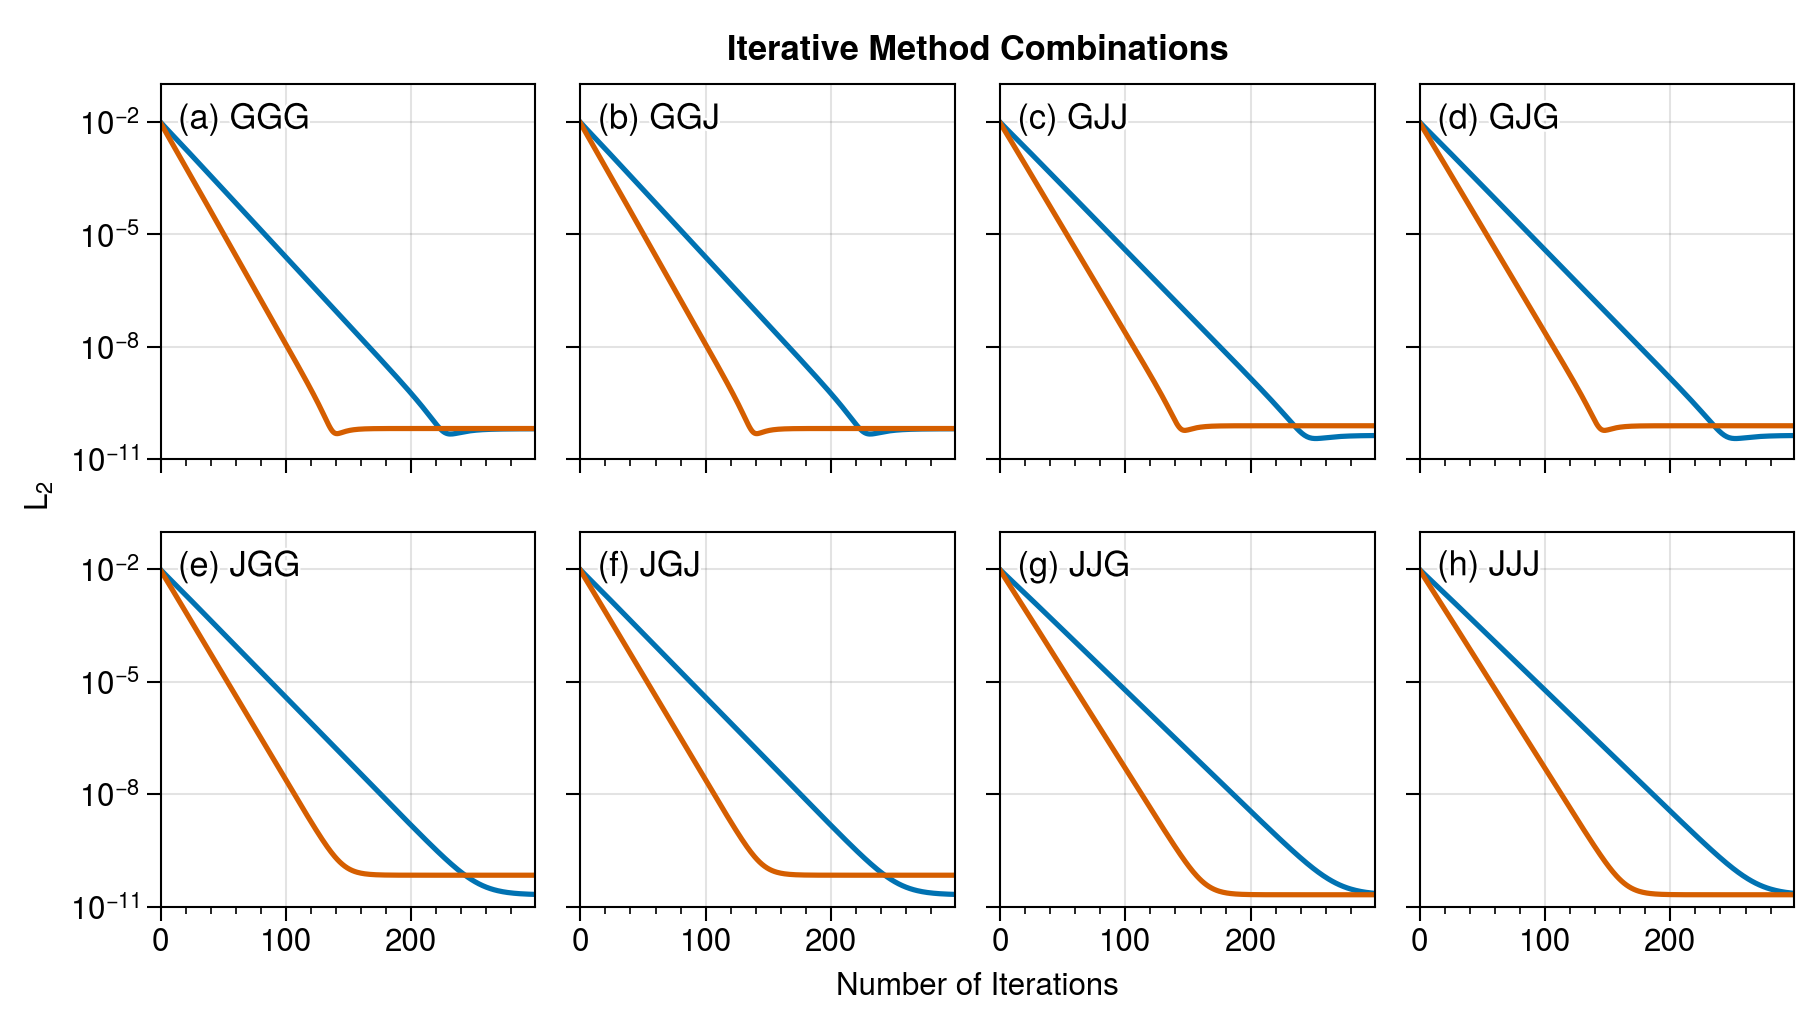
\includegraphics[width=\textwidth]{figures/prj1_qn2c_pt1.png}\\
    \caption{The $L_2$ norm of $\phi$ for the different combinations of the Gauss-Seidel and Jacobi methods.  The order is given in Restriction-Prolongation-Coarse, with "G" representing Gauss-Seidel and "J" representing Jacobi iterative methods respectively.  Blue represents $\omega = 0.5$ and red represents $\omega = 0.8$ relaxation factors respectively.}
    \label{prj1_qn2c_pt1}
    \end{figure*}
    
    We see that the Gauss-Seidel method causes a faster convergence than the Jacobi method when it is used in the relaxation of $\nu_1$ and $\nu_2$ methods.  This is particularly obvious when the relaxation factor $\omega$ is small.  Whether Gauss-Seidel or Jacobi methods are used in the iteration of the coarse grid does not seem to make any significant difference in the convergence rate.  Obviously, we see that higher relaxation factors are better for the multigrid routine.
    
    Next, we proceed to vary $\nu_c$, or the number of coarse-grid iterations, in our multigrid.  We do $\nu_c = 2,4,10,20,50$ and an exact solution which is derived from a direct solve of the matrix equation $A\mathbf{e}=r$ on the coarse grid (Fig. \ref{prj1_qn2c_pt2}).  As $\nu_c$ increases, we see that $\phi$ converges to the exact solution found from the direct solve much faster.  In fact, at $\nu_c = 50$, we see that $\phi$ converges within 10 iterations when $\omega = 0.8$.

    \begin{figure*}[h!]
    \centering
    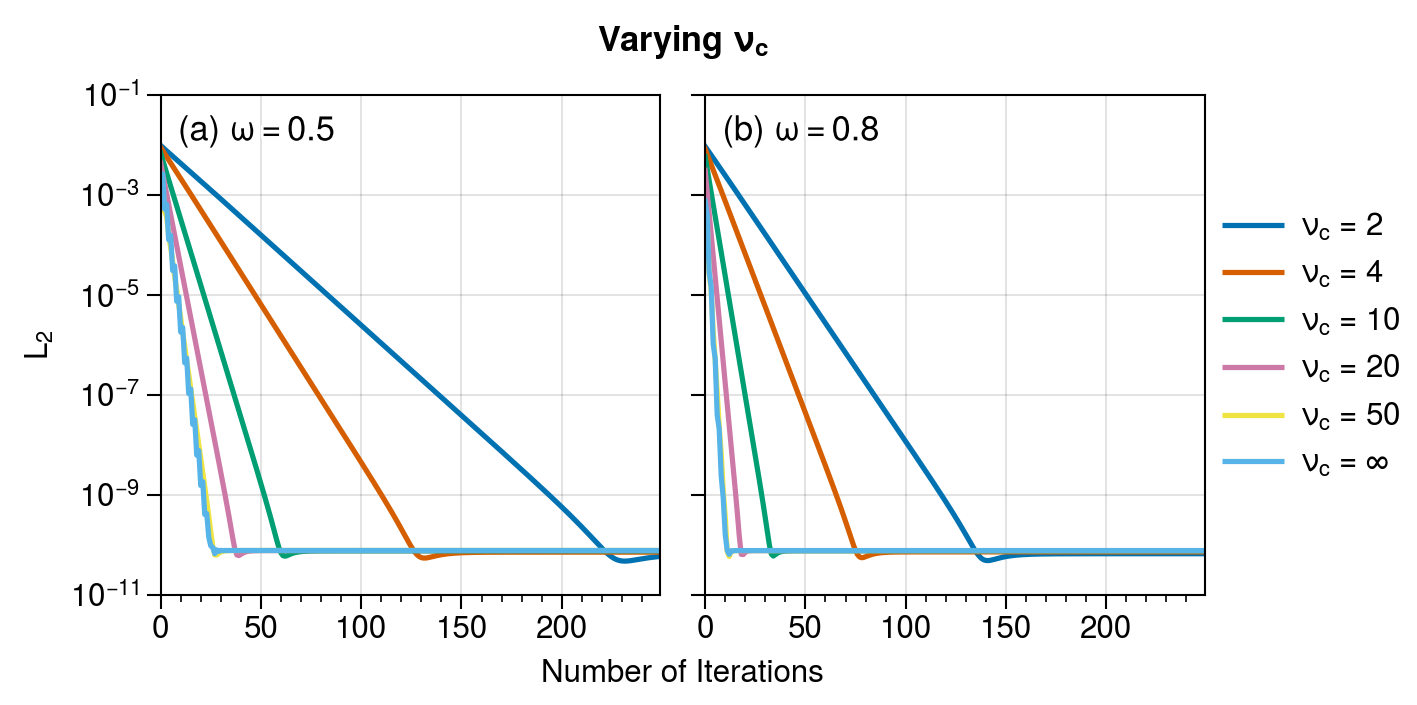
\includegraphics[width=0.7\textwidth]{figures/prj1_qn2c_pt2.png}\\
    \caption{The $L_2$ norm of $\phi$ for the different combinations of the Gauss-Seidel and Jacobi methods.  The order is given in Restriction-Prolongation-Coarse, with "G" representing Gauss-Seidel and "J" representing Jacobi iterative methods respectively.  Blue represents $\omega = 0.5$ and red represents $\omega = 0.8$ relaxation factors respectively.}
    \label{prj1_qn2c_pt2}
    \end{figure*}
    
    \item Using $\nu_1=\nu_2 = 1$, $\nu_c=50$, we iterate over all the possible configurations of the source blocks, and find that the configuration is [1,6,11,14].  We see the table below for the fluxes we solved, and Fig. \ref{prj1_qn2d} for the distribution of $\phi$ resulting from this configuration.

    \begin{figure*}[h!]
    \centering
    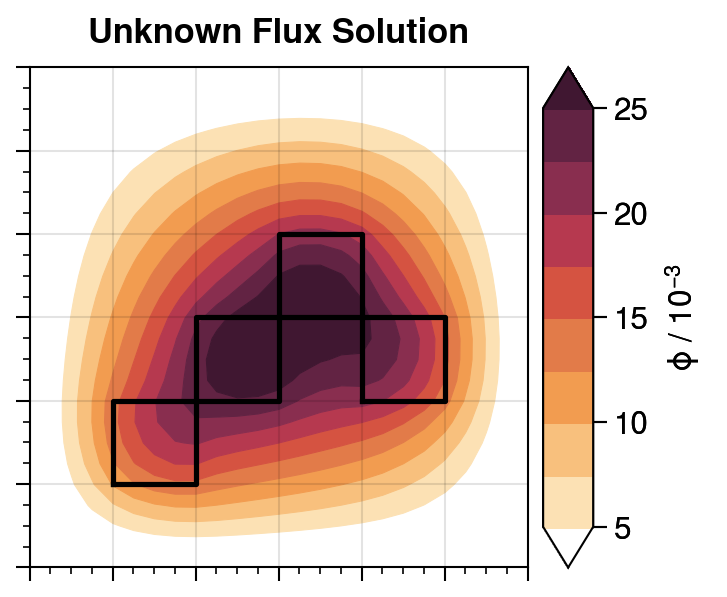
\includegraphics[width=0.4\textwidth]{figures/prj1_qn2d.png}\\
    \caption{The spatial distribution of $\phi$ where $\partial_n\phi$ matches the unknown flux boundaries in the question.  The source blocks are [1,6,11,14].}
    \label{prj1_qn2d}
    \end{figure*}
    
    \begin{lstlisting}
 ------ ------------ ------------ ------------ ------------
  Node      Left        Right        Bottom        Top     
 ------ ------------ ------------ ------------ ------------
  1.0       0.0          0.0          0.0          0.0
  2.0    0.0140286    0.00840473   0.0140449    0.00493154
  3.0    0.0279173    0.0169555    0.0279824    0.00984111
  4.0     0.041279    0.0257883    0.0414581    0.0147044
  5.0    0.0533502    0.0350073    0.0537404    0.0194921
  6.0    0.0633332    0.0446356    0.0640629    0.0241674
  7.0    0.0704305     0.054519    0.0716577    0.0286823
  8.0    0.0742918    0.0641842      0.0762     0.0329741
  9.0    0.0750902    0.0727668    0.0778825    0.0369615
  10.0   0.0734799    0.0793828    0.0773693    0.0405407
  11.0   0.0701791    0.0831751     0.075374    0.0435845
  12.0   0.0659514    0.0837638    0.0726351    0.0459471
  13.0   0.0612513    0.0813218    0.0695556    0.0474778
  14.0   0.0562948    0.0765273    0.0662672    0.0480426
  15.0   0.0511854    0.0701388    0.0627537    0.0475489
  16.0   0.0459857    0.0629683    0.0589274    0.0459657
  17.0    0.040744    0.0555178    0.0546704    0.0433314
  18.0   0.0354992    0.0480418    0.0498644     0.039746
  19.0   0.0302809    0.0406661    0.0444187    0.0353509
  20.0   0.0251087    0.0334561    0.0382943    0.0303042
  21.0   0.0199926    0.0264415    0.0315148    0.0247593
  22.0   0.0149334     0.019623    0.0241624    0.0188517
  23.0   0.00992434   0.0129758    0.0163608    0.0126953
  24.0   0.00495234   0.00645461   0.00825606   0.00638449
  25.0      0.0          0.0          0.0          0.0
 ------ ------------ ------------ ------------ ------------
\end{lstlisting}
    
    \item Lastly, we generalize a V-cycle multigrid routine which allows for multiple grid refinements.  Since a 4-grid refinement is technically not possible for a 25-node grid (it can only go down two levels to 13 and 7 while keeping resolution for 6 source blocks), we start with a 49-node grid.  We take $\nu_1=\nu_2 = 1,2$, $\nu_c=2,5,10$.  We vary $\nu_n$, or the number of refinements, from 2-4, and plot our results in Fig. \ref{prj1_qn2e}.
    
    We see that higher $\nu_n$ results in a faster convergence.  However, we also see that as $n\nu_n$ increases, the likelihood of instability also increases and requires more relaxation iterations $\nu_1$ and/or $\nu_2$ for smoothing.

    \begin{figure*}[h!]
    \centering
    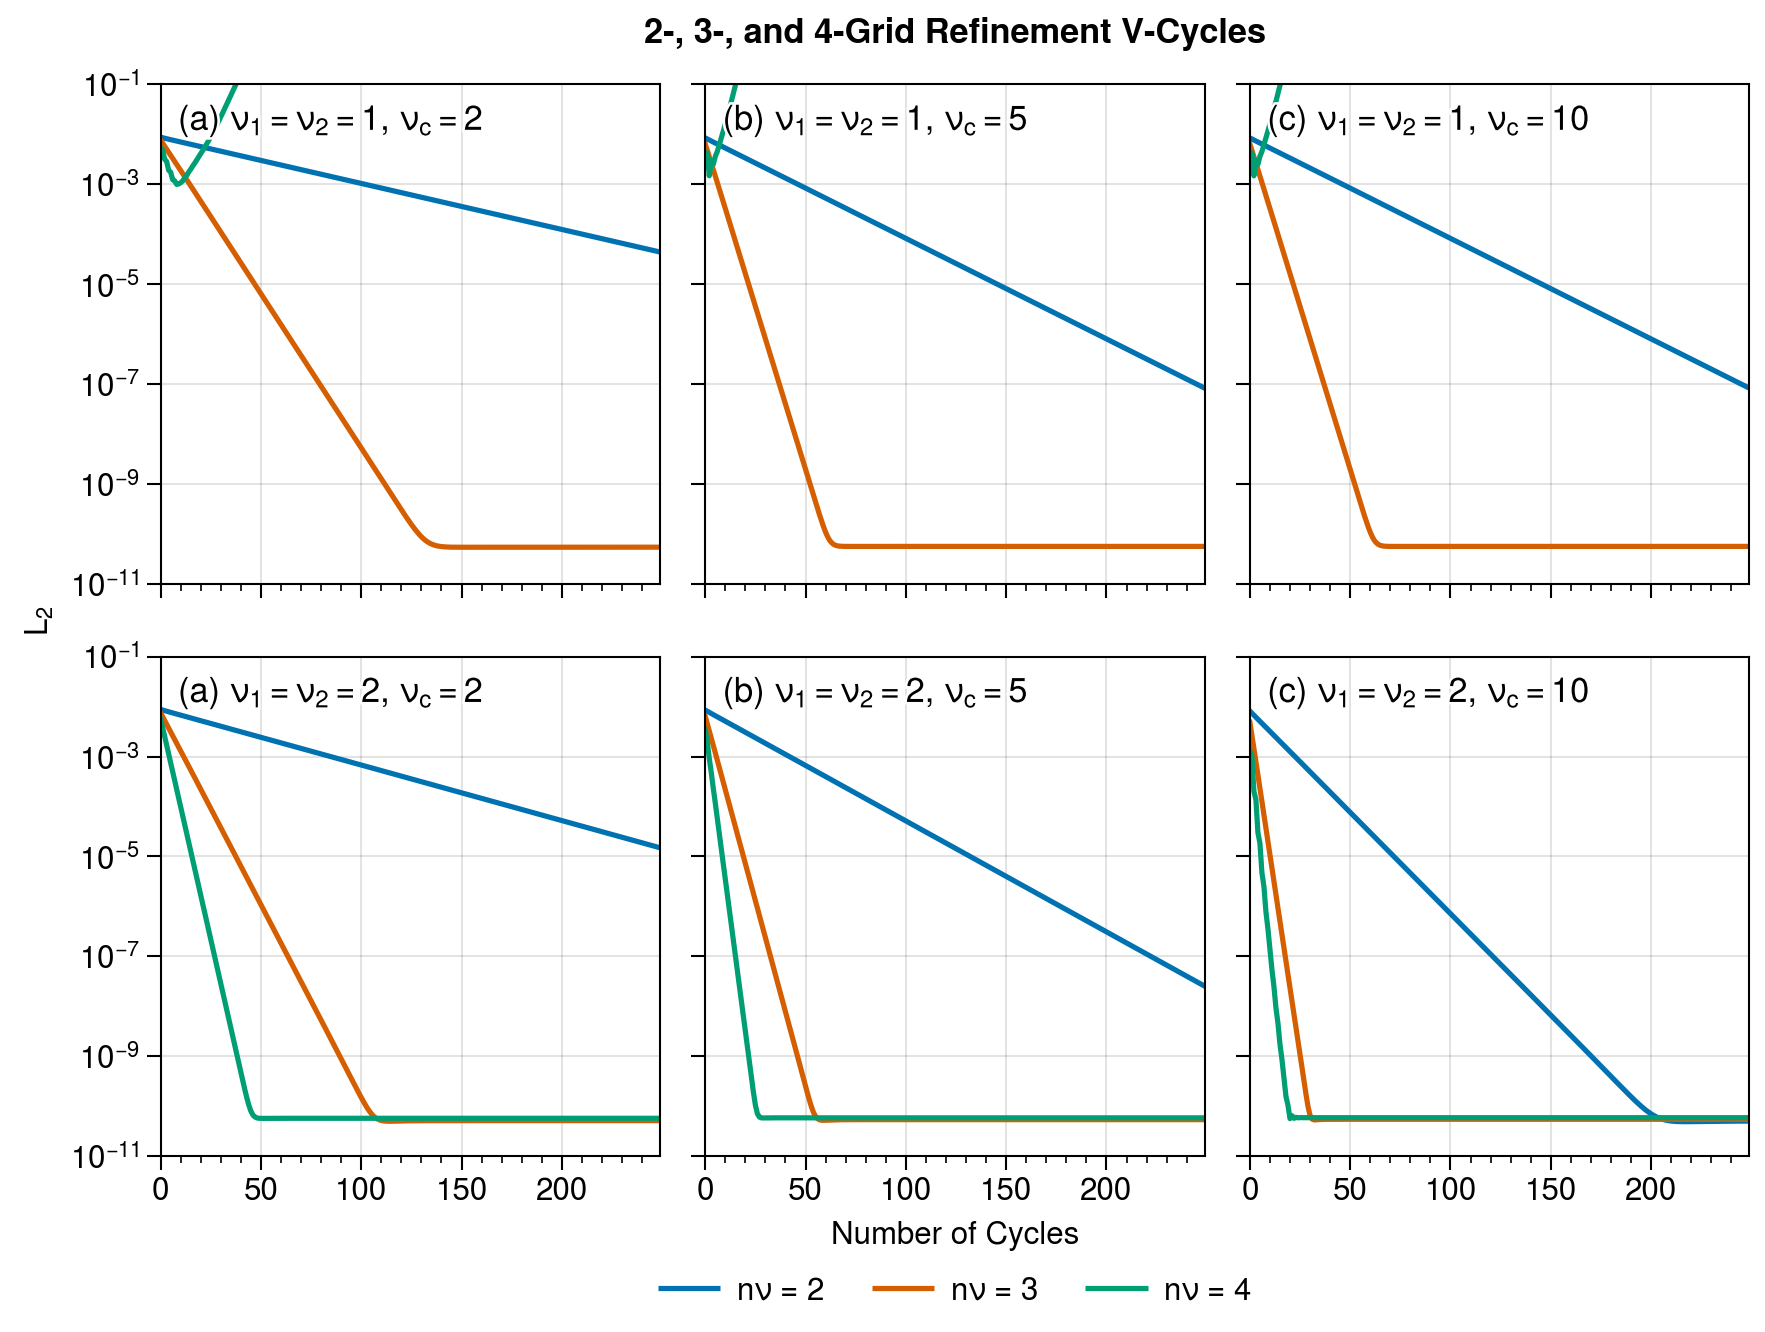
\includegraphics[width=\textwidth]{figures/prj1_qn2e.png}\\
    \caption{The $L_2$ norm of $\phi$ over 250 cycles for $\nu_n = 2,3,4$ for (top) $\nu_1=\nu_2=1$, (bottom) $\nu_1=\nu_2=2$ and (left) $\nu_c=2$, (center) $\nu_c=5$, (right) $\nu_c=10$.  We see that higher $\nu_n$ requires higher $\nu_1$, $\nu_2$ for better smoothing to prevent instability as the cycles progress.}
    \label{prj1_qn2e}
    \end{figure*}
    
\end{enumerate}